\documentclass[11pt]{article}
\usepackage{a4wide,parskip,times}
\usepackage{graphicx, caption}
\usepackage{booktabs}
\usepackage{cite}
\usepackage{longtable}

\begin{document}

\centerline{\Large Super-Resolution on Light Field Data}
\vspace{2em}
\centerline{\Large \emph{An MPhil project proposal}}
\vspace{2em}
\centerline{\large D. Yue (\emph{dy276}), Magdalene College}
\vspace{1em}
\centerline{\large Project Supervisor: Dr R. Mantuik}
\vspace{1em}

\begin{abstract}
  Light field image data has been used in many applications including post
  capture image refocusing or 3D image display. Thanks to the commercialisation
  of the light field camera, we could foresee the light field data massively
  available in the near future. However, due to the fundamental trade-off
  between the spatial and angular resolution, computational approach to increase
  the resolution of raw data is desired. For this project, I propose to survey
  the method on the light field super resolution, particularly in angular domain
  and implement an application with statistical approach.
\end{abstract}

\section{Introduction, approach and outcomes}

\subsection*{Light Field and Light Camera}

Light field is a 4D vector field that measures the intensity of the light given
the spatial coordinates and angular direction. Comparing with traditional 2D
images, light field has the ability to (1) render images with with post-capture
control of focus and depth-of-field\cite{ng2005light}, (2) render images from
different viewpoints\cite{ng2005light} within a range without extra depth
information or feature matching (3) construct real 3D images without effect of
visual contractions.\cite{wetzstein2012tensor}

Thanks to recent commercialisation of light field camera\cite{georgiev2013lytro},
capturing a dense camping of the light field became feasible for real world
applications. However, light field camera with modest sensor often face the
trade-off between spatial and angular resolution - either sample densely in the
spatial domain and sparsely in the angular domain or vice versa. Thus, there are
great interests to increase resolution of the raw captured light field sampling
with computational method.

\begin{figure}
  \centering
  \captionsetup{width=0.8\linewidth}
  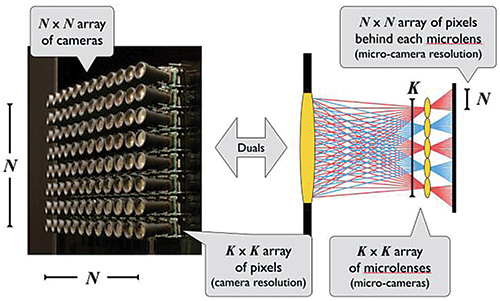
\includegraphics[width=0.8\textwidth]{./light-field-trade-off.jpg}
  \caption{
    Image provided by \cite{imtradoff}, it shows how two different design of
    light field camera trade off between spatial and angular resolution, while
    the camera system on the left has spatial resolution of $K^2$ and angular
    resolution of $N^2$, the camera system on the right has spatial resolution
    of $N^2$ and angular resolution fo $K^2$
  }
\end{figure}

\subsection*{Super Resolution Techniques}

Super resolution refers to a class of techniques that enhance the resolution of
an imaging system. For light field system, one would enhance the resolution
either in spatial domain or in angular domain.

Spatial super resolution of light field images could be regarded as a special
case for constructing high resolution image from multiple low resolution images.
And the angular super resolution is equivalent to the synthesis of novel view
from new viewpoints.

Comparing with more generalized super-resolution problems, light field data have
several advantages for super resolution tasks: 1) the camera position is known
2) the camera positions are regularly distributed on the grid 3) A decent amount
of relevant images are available. Thus, many techniques that are specific to the
light field data has been proposed. To the best of my knowledge, these
techniques could be categorised into three major ways.  To best of my knowledge,
the super-resolution techniques for light field could be roughly divided into
three categories.

\begin{enumerate}

  \item Statistical method by the restoration techniques\cite{mitra2012light}
    \cite{wanner2014variational} \cite{rossi2017graph} : The low resolution
    sampling was treated as the product of the noise and down-sample operator
    from the high resolution light field.

  \item Learning base methods\cite{yoon2017light} \cite{gul2017spatial}: some
    have also successfully tried to use popular deep learning techniques to train
    an end to end convolutional neural network.

  \item Hybrid image system\cite{boominathan2014improving}: some tried to use
    a hight spatial resolution camera in addition to the light field camera to
    enhance the spatial resolution of the light field data.

\end{enumerate}

\subsection*{Approach}


\cite{georgiev2006spatio} has argue that trading off with dense sampling of the
spatial resolution and sparse sampling of the angular resolution is essential
for camera space in integral photography. Thus, by following this argument, I
plan to implement an algorithm to increase the angular resolution given the
light field data under the statistical framework view stated as above.

\begin{figure}[t]
  \centering
  \captionsetup{width=0.8\linewidth}
  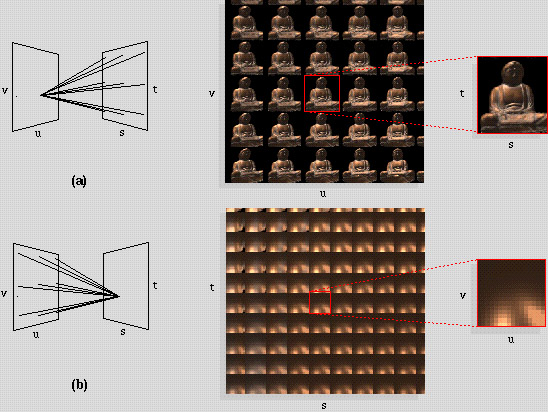
\includegraphics[width=0.8\textwidth]{./light-field-slice.jpg}
  \caption{
    Image from \cite{levoy1996light}. Light field data could be viewed as a 4D
    array $L(u, v, s, t)$ where two dimension $(u, v)$ paramatrise the angular
    variation and $(s, t)$ paramatrise the spatial variation. The right top shows
    the spatial slices if we fix $(u, v)$ and the right bottom shows the angular
    slices if we fix $(s, t)$
  }
\end{figure}

I plan to follow the following pipeline.

\begin{itemize}
  \item Find depth estimation of spatial slices of each angular resolution
  \item Register the corresponding points between each spatial slices
  \item Warp the registered images the specified angular direction
  \item Refinement from the current estimation
\end{itemize}

During this process, many factors including noise, occlusion and non-lambertian
surface will present challenges to the quality of our super resolution
algorithm. Thus, this project will also investigate if the specific properties
of light field could be utilised to achieve better result in these challenging
settings.

\section{Work plan}

The work has been divided into 2 weeks chunk for total of 14 chunks. The
detailed plan is listed as below. I will count one week as 5 days and weekends
would be reserved for emergencies only.

\begin{longtable}{|p{0.15\textwidth}|p{0.3\textwidth}|p{0.55\textwidth}|}
  \caption{\textbf{Work Plan}}\\
  \hline
  Week & Milestone & General Description \\ \hline

  04/12-17/12 Week 0-1&
  Prepare the experimental data &
  \begin{itemize}
    \item collect light field dataset from the internet (2days)
    \item generate the light field data from 3D model, to obtain ground truth in
      depth estimation, image registration and interpolated scene for future
      analysis.(3days)
    \item Devoted to course work (mini-projects). (5 days)
  \end{itemize}
  \\ \hline
  08/12-31/12 Week 2-3&
  None &
  \begin{itemize}
    \item Devoted to course work (mini-projects). (10 days)
    \item Reading relevant techniques used for density
      estimation, warping frames \cite{huang2017robust} \cite{li2017robust}
      in spare time.
  \end{itemize}
  \\ \hline

  01/01-14/01 Week 4-5&
  None &
  \begin{itemize}
    \item Devoted to course work (mini-projects). (10 days)
    \item same as above
  \end{itemize}
  \\ \hline

  05/01-28/01 Week 6-7&
  Implement on the basic naive estimation stage and image registration stage &
  \begin{itemize}
    \item Try naive implementation on depth estimation with two view geometry
      and multiple view geometry. (6 days)
    \item Try naive implementation on image registration with feature matching.
      (4 days)
  \end{itemize}
  \\ \hline

  09/01-11/02 Week 8-9&
  Implement the wrap stage and first naive implement of the whole pipeline &
  \begin{itemize}
    \item Implement the naive warping algorithm given the image registration
      result. (3 days)
    \item Implement the naive warping algorithm given the depth estimation
      result (3 days)
    \item Connect the whole pipeline and evaluate the result. (4 days)
  \end{itemize}
  \\ \hline

  02/02-25/02 Week 10-11&
  Improve the naive solution with better depth estimation &
  \begin{itemize}
    \item Choose to follow a better algorithm for depth estimation related to
      light field. \cite{jeon2015accurate} \cite{wang2016depth} (10 days)
  \end{itemize}
  \\ \hline

  06/02-11/03 Week 12-13&
  Improve the naive solution with better registration techniques &
  \begin{itemize}
    \item Choose a registration techniques specific to light field.
      \cite{mukati2016light}
  \end{itemize}
  \\ \hline

  02/03-25/03 Week 14-15&
  Improve the naive solution with better wrap scheme &
  \begin{itemize}
    \item Implement a better warping algorithm by treating the problem as the
      image restoration task (MAP frame and energy minimisation).
      \cite{rossi2017graph} (10 days)
  \end{itemize}
  \\ \hline

  06/03-08/04 Week 16-17&
  Improve the application with refinement post process &
  \begin{itemize}
    \item Investigate techniques for post-process improvement. (10 days)
  \end{itemize}
  \\ \hline

  09/04-22/04 Week 18-19&
  Finish the first draft on chapters of introduction / background / related work
  &
  \begin{itemize}
    \item write introduction (2 days)
    \item write background information (3 days)
    \item summarise the related work (4 days)
    \item collect experiment result from datasets (1 day)
  \end{itemize}
  \\ \hline

  03/04-06/05 Week 20-21&
  Finish the first draft on chapters of methodology &
  \begin{itemize}
    \item prepare additional experiment result from datasets (2 days)
    \item write methodology sections (3 days)
    \item write experiment sections (5 days)
  \end{itemize}
  \\ \hline

  07/05-20/05 Week 22-23&
  Finish the first draft of the dissertation. &
  \begin{itemize}
    \item write conclusion and result the first draft. (3 days)
    \item extension on more efficient algorithm (7 days)
  \end{itemize}
  \\ \hline

  01/05-03/06 Week 24-25&
  Finalise the dissertation. &
  \begin{itemize}
    \item Finalise the dissertation (10 days)
  \end{itemize}
  \\ \hline

  04/06-10/06 Week 26&
  None &
  Reserved for emergencies.
  \\ \hline
\end{longtable}


\newpage
\appendix
\bibliographystyle{unsrt}
\bibliography{proposal}
\end{document}
